\thispagestyle{fancy}
\vspace*{0cm} % move text up to start near top of page

\section{Data Exchanged Between the Control and Station Laptops}

Building on the communication architecture established in the previous chapter, this section details the concrete payloads that traverse the link between the two nodes during operation. The exchange is bidirectional but asymmetric: the station laptop, which is co-located with the cameras and the physical manipulators, streams perception and state information \textit{up} to the control laptop, while the control laptop --- which performs the planning and trajectory generation --- sends the resulting execution program \textit{down} to the station for the robots to carry out. The two directions use \textit{different transport mechanisms suited to their data}: the station's live telemetry is streamed over ROS2 topics, each matched across the ZeroTier overlay through the unicast Fast~DDS discovery described earlier, whereas the control laptop's planned program is delivered as a file through \textbf{Syncthing}, a continuous file-synchronization service running over the same overlay.

\begin{figure}[htbp]
    \centering
    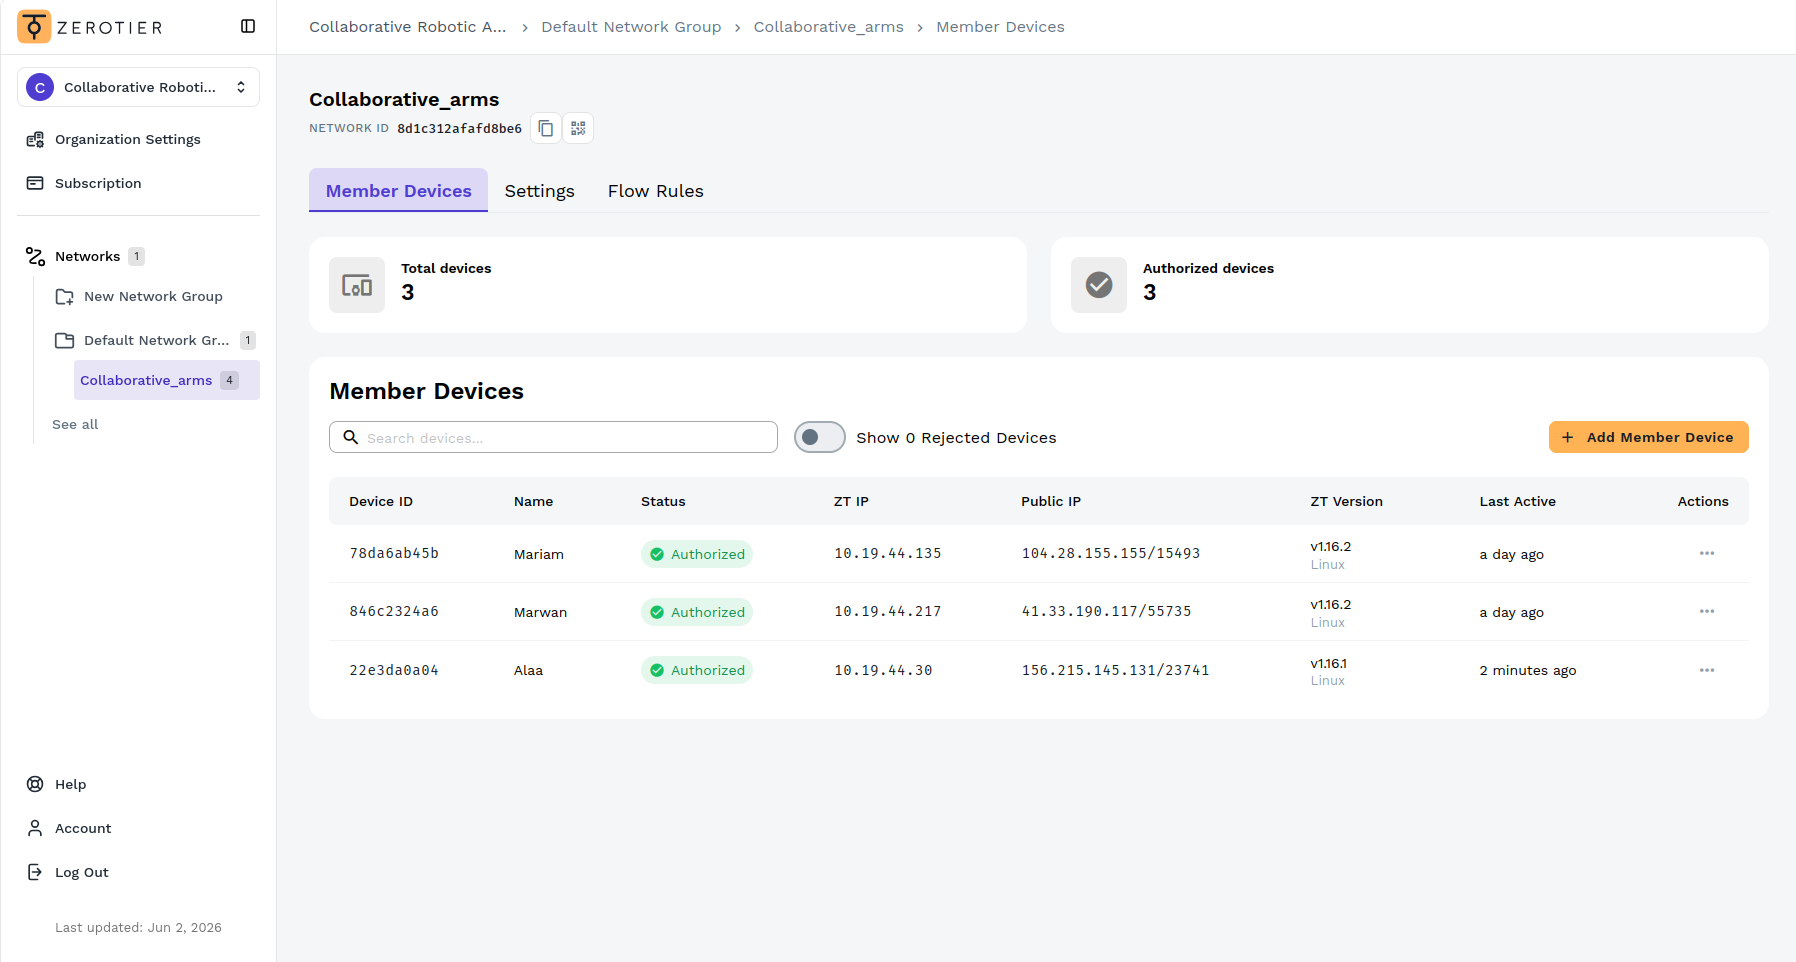
\includegraphics[width=0.9\textwidth]{figures/chapter6/iot/zero_tier.png}
    \caption{Zerotier UI}
    \label{fig:zerotier_ui}
\end{figure}

\subsection{Station Laptop \texorpdfstring{$\rightarrow$}{->} Control Laptop}

The station laptop is the source of all real-world observations fed back into the planning loop. It publishes three categories of data:

\begin{itemize}
    \item \textbf{Brick detections from the camera.} The vision pipeline running on the station laptop processes the camera feed and publishes the detected bricks --- their identities and estimated poses --- to the control laptop. This is the perception input from which the control laptop builds its world model and decides which bricks to pick and where to place them.
    \item \textbf{Joint states of the physical arms (\texttt{/joint\_states}).} The measured joint positions of the real ABB and AR4 manipulators are streamed continuously so that the control laptop and its digital twin remain synchronized with the true state of the hardware. This feedback closes the loop between the planned motion and the actual configuration of the arms.
    \item \textbf{System status flags.} A set of lightweight status messages communicates the current operational state of the station --- for example, the active phase of the assembly cycle and readiness or fault conditions --- allowing the control laptop to sequence its commands against the real progress of the cell.
\end{itemize}

\subsection{Control Laptop \texorpdfstring{$\rightarrow$}{->} Station Laptop}

In the opposite direction, the control laptop sends a single but information-dense payload:

\begin{itemize}
    \item \textbf{The program storage.} Once the control laptop has planned the task, it produces the \textit{program storage} --- a structured \texttt{YAML} file holding the trajectories that the robots are to execute. This file encodes the planned motion for the manipulators and constitutes the command program that drives the physical execution on the station side.
\end{itemize}

Unlike the station's telemetry, the program storage is not a continuous stream of small messages but a single, self-contained document that is regenerated whenever the plan changes. This makes it a poor fit for a publish--subscribe topic and a natural fit for file synchronization, which is why it is delivered with Syncthing rather than over a DDS topic.

\subsection{Program-Storage Transfer with Syncthing}

\textbf{Syncthing} is an open-source, peer-to-peer continuous file-synchronization application. Rather than transferring files on explicit request, it keeps a designated folder identical across two or more devices: whenever a file in that folder changes on one device, the change is detected and propagated to every other device sharing the folder. There is no central server --- each device communicates directly with its peers --- and all traffic between them is encrypted end-to-end using TLS, with every device identified by a unique cryptographic device ID.

In this system, a single \textit{shared folder} is configured on both the control and the station laptops. The control laptop writes the program-storage \texttt{YAML} file into this folder, and Syncthing automatically transfers the updated file to the station laptop, where the execution process reads it. The transfer proceeds as follows:

\begin{enumerate}
    \item \textbf{Folder sharing.} The folder containing the program storage is added to Syncthing on the control laptop and shared with the station laptop's device ID; the station accepts the share, establishing a synchronized folder pair.
    \item \textbf{Change detection.} Syncthing continuously watches the folder. When the control laptop regenerates the program-storage file after planning, the modification is detected almost immediately through filesystem-change notifications.
    \item \textbf{Indexing and block transfer.} The modified file is split into blocks; Syncthing exchanges an updated index with the peer and transfers only the blocks that have actually changed, which keeps successive updates efficient. The new version then atomically replaces the old file on the station side, so the station never reads a half-written file.
    \item \textbf{Peer connectivity.} Because both laptops are members of the same ZeroTier overlay, Syncthing establishes its direct, encrypted peer connection over the stable virtual IP addresses, in the same way the DDS traffic does. The synchronization therefore works across the two physical networks without any additional port forwarding or relay configuration.
\end{enumerate}

This arrangement cleanly separates the two kinds of traffic: time-critical, high-rate telemetry travels over the real-time DDS link, while the larger, infrequently-updated program file is handled by a service purpose-built for reliable file delivery. Syncthing also provides versioning and automatic recovery from interrupted transfers, so a dropped connection during an update simply resumes once connectivity is restored, without corrupting the file the station relies on.

% PLACEHOLDER: Data-exchange flow diagram between the two laptops
\begin{figure}[htbp]
    \centering
    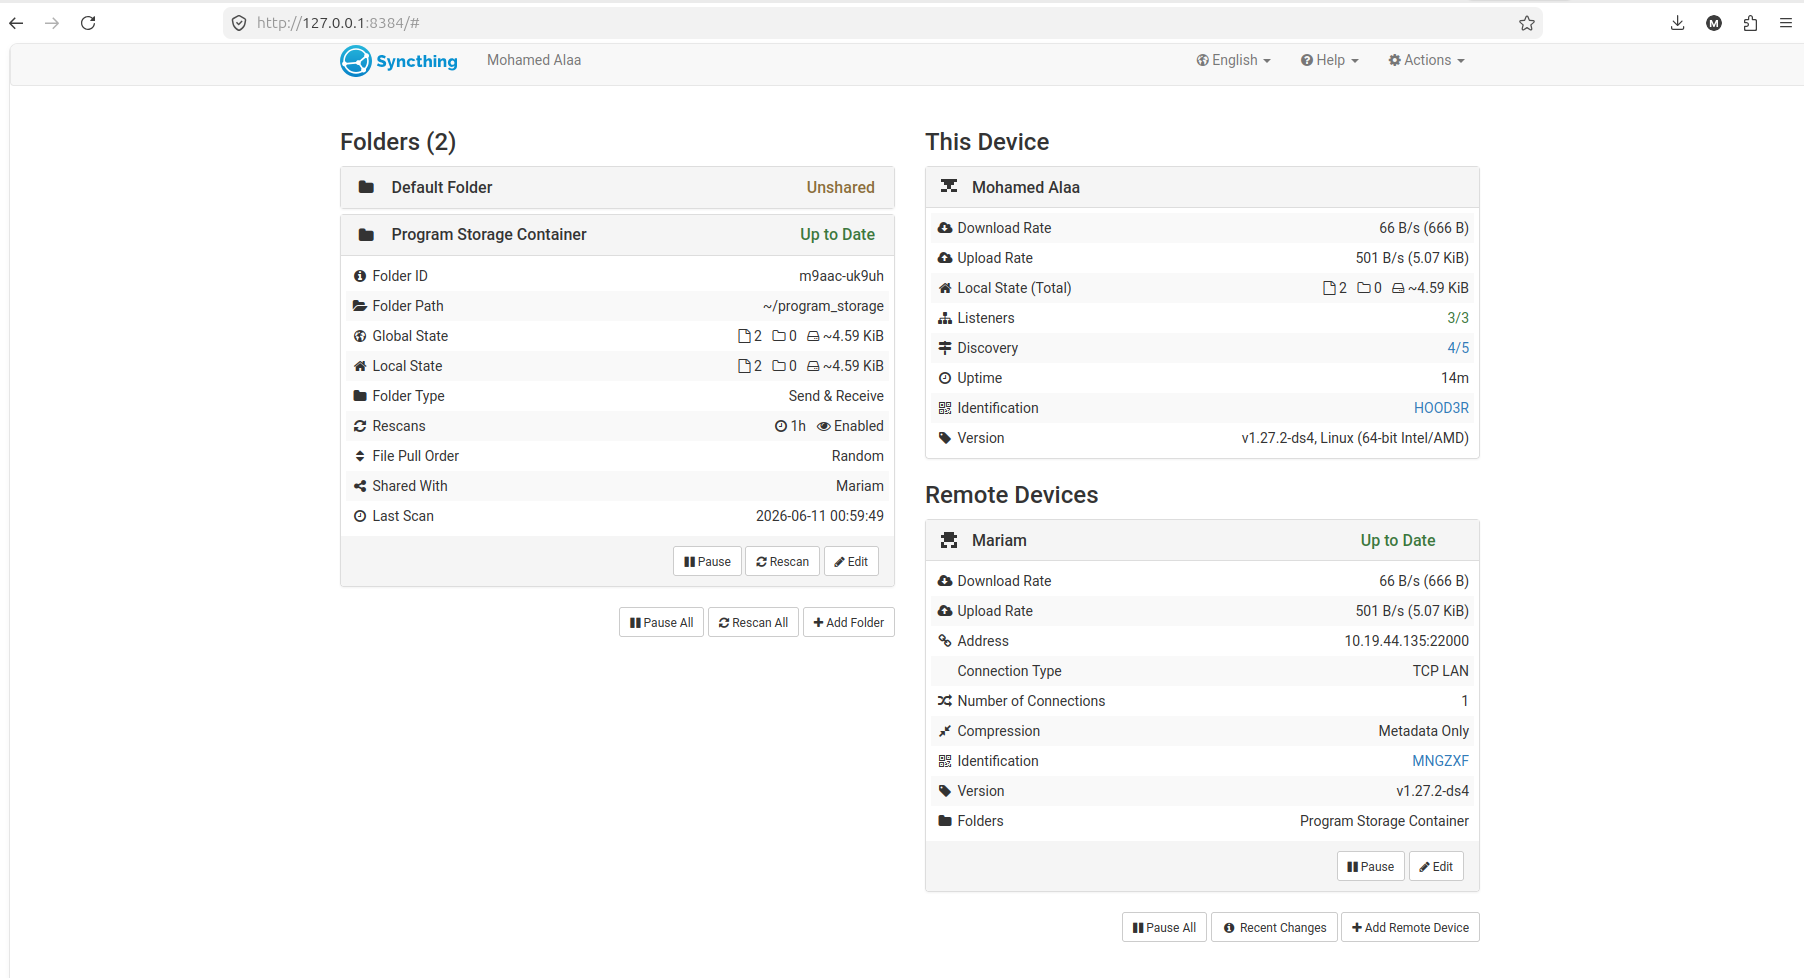
\includegraphics[width=0.9\textwidth]{figures/chapter6/iot/syncthing_2.png}
    % \rule{0.9\textwidth}{6cm} % Placeholder box
    \caption{Syncthing Folder Exchange UI.}
    \label{fig:syncthing_ui}
\end{figure}

\subsection{Summary of the Data Flow}

The complete set of payloads exchanged across the link is summarized below and illustrated in Figure~\ref{fig:data_exchange_flow}. The asymmetry of the exchange reflects the division of responsibility: perception and ground-truth state originate at the station, while the planned trajectories originate at the control node.

\medskip
\noindent\textbf{Station laptop $\rightarrow$ Control laptop (over ROS2 / Fast~DDS):}
\begin{itemize}
    \item Brick detections from the camera --- identities and poses of detected bricks (perception input for planning).
    \item Joint states (\texttt{/joint\_states}) --- real-time joint feedback from the physical ABB and AR4 arms (synchronizes the digital twin).
    \item System status flags --- current operational state of the cell (used for command sequencing).
\end{itemize}

\noindent\textbf{Control laptop $\rightarrow$ Station laptop (over Syncthing):}
\begin{itemize}
    \item Program storage (\texttt{YAML}) --- the planned trajectories for the robots to execute.
\end{itemize}

% PLACEHOLDER: Data-exchange flow diagram between the two laptops
\begin{figure}[htbp]
    \centering
    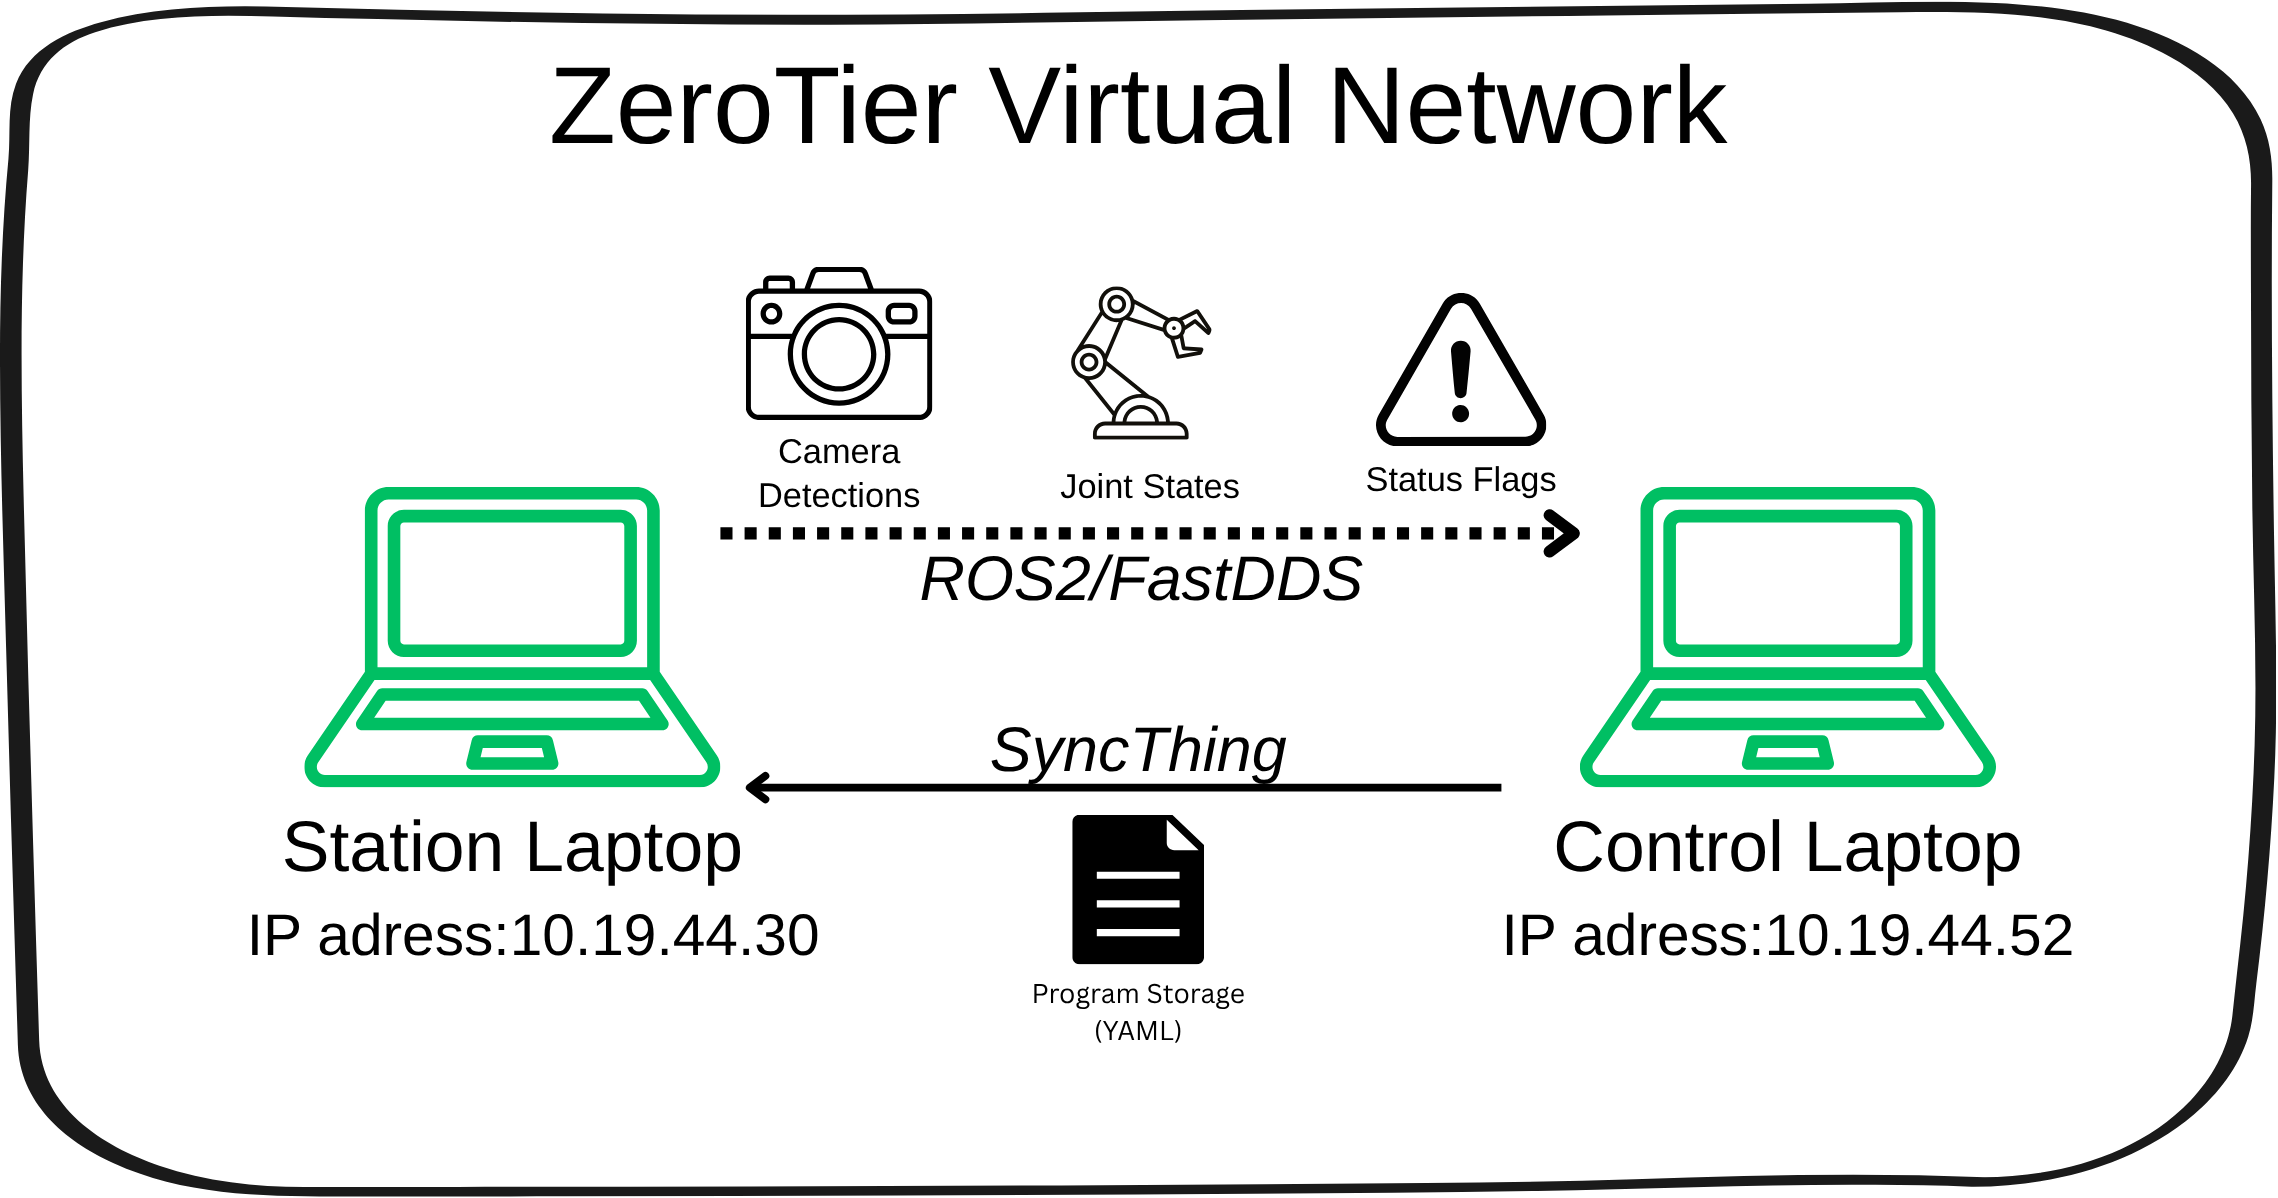
\includegraphics[width=0.9\textwidth]{figures/chapter6/iot/data_flow2.png}
    % \rule{0.9\textwidth}{6cm} % Placeholder box
    \caption{Data-exchange flow between the control and station laptops.}
    \label{fig:data_exchange_flow}
\end{figure}